% Example preprint (synthetic, fictional). Build: latexmk -pdf main.tex
% Every number comes from paper/values.toml through \val{key}; regenerate with `steward paper values --write`.
\documentclass[11pt]{article}
\usepackage[T1]{fontenc}
\usepackage{booktabs}
\usepackage{tikz}
\usepackage[numbers]{natbib}
\usepackage{hyperref}
% Generated by `steward paper values --write`. Do not edit; regenerate after results change.
% Use \val{key} in the text. An unknown key stops the build with an error.
\makeatletter
\providecommand{\val}[1]{\@ifundefined{stewardval@#1}{\PackageError{steward}{Unknown value key #1}{Add it to values.toml}}{\@nameuse{stewardval@#1}}}
\@namedef{stewardval@alpha}{0.05}
\@namedef{stewardval@min_gain}{0.05}
\@namedef{stewardval@n_donors}{40}
\@namedef{stewardval@n_samples}{120}
\@namedef{stewardval@n_test_donors}{8}
\@namedef{stewardval@n_test_samples}{24}
\@namedef{stewardval@n_train_donors}{24}
\@namedef{stewardval@n_train_samples}{72}
\@namedef{stewardval@n_val_donors}{8}
\@namedef{stewardval@n_val_samples}{24}
\@namedef{stewardval@resamples}{2000}
\@namedef{stewardval@samples_per_donor}{3}
\makeatother


\title{Donor-level splits for a synthetic responder benchmark}
\author{Example Author}
\date{}

\begin{document}
\maketitle

\begin{abstract}
Benchmarks with several samples per donor can report optimistic scores when samples of one donor fall in both the
training and the test split. We describe a donor-level evaluation design for a synthetic responder-classification
task, fixed before any model is trained. This document reports the design only; results will follow a declared
comparison procedure.
\end{abstract}

\section{Introduction}\label{sec:intro}
Donor-aware models have been proposed for expression data \citep{exampleA2025}, and logistic regression remains a
common baseline \citep{exampleC2024}. Section~\ref{sec:methods} states the design and Section~\ref{sec:limits} its
limitations.

\section{Benchmark design}\label{sec:methods}
The synthetic dataset has \val{n_donors} donors with \val{samples_per_donor} samples each. All samples of a donor are assigned to one split
(Table~\ref{tab:splits}, Figure~\ref{fig:donors}). The primary metric is the area under the ROC curve, compared with a paired bootstrap (\val{resamples} resamples,
$\alpha = \val{alpha}$); the candidate must exceed logistic regression by at least \val{min_gain}.

\begin{table}[t]
\centering
\caption{Donor-level splits.}\label{tab:splits}
% Generated by analysis/make_displays.py table; do not edit.
\begin{tabular}{lrr}
\toprule
Split & Donors & Samples \\
\midrule
Train & 24 & 72 \\
Validation & 8 & 24 \\
Test & 8 & 24 \\
\bottomrule
\end{tabular}

\end{table}

\begin{figure}[t]
\centering
% Generated by analysis/make_displays.py figure; do not edit.
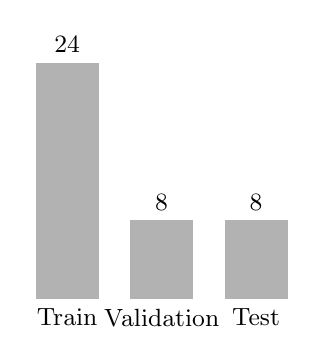
\begin{tikzpicture}
\fill[gray!60] (0.0,0) rectangle (0.8,3.000);
\node[below] at (0.4,0) {\small Train};
\node[above] at (0.4,3.000) {\small 24};
\fill[gray!60] (1.2,0) rectangle (2.0,1.000);
\node[below] at (1.6,0) {\small Validation};
\node[above] at (1.6,1.000) {\small 8};
\fill[gray!60] (2.4,0) rectangle (3.2,1.000);
\node[below] at (2.8,0) {\small Test};
\node[above] at (2.8,1.000) {\small 8};
\end{tikzpicture}

\caption{Donors per split.}\label{fig:donors}
\end{figure}

\section{Limitations}\label{sec:limits}
The data are synthetic and carry no biological meaning. No results are reported at this stage.

\section*{Competing interests}
None (fictional example).

\bibliographystyle{plainnat}
\bibliography{refs}
\end{document}
